\documentclass[tikz,border=3pt]{standalone}
\usepackage[T1]{fontenc}
\usepackage[scaled=0.92]{helvet}
\renewcommand{\familydefault}{\sfdefault}
\usepackage{amsmath,amssymb}
\usetikzlibrary{arrows.meta,positioning,calc,decorations.pathreplacing}

\definecolor{ink}{HTML}{27313D}
\definecolor{muted}{HTML}{5F6C79}
\definecolor{grid}{HTML}{D7DCE2}
\definecolor{panelgray}{HTML}{F7F8FA}
\definecolor{gold}{HTML}{F2C66D}
\definecolor{goldline}{HTML}{C98A20}
\definecolor{direct}{HTML}{3569AD}
\definecolor{directlight}{HTML}{EAF1F9}
\definecolor{cot}{HTML}{347E68}
\definecolor{cotlight}{HTML}{E8F3EF}
\definecolor{transition}{HTML}{7154B3}
\definecolor{transitionlight}{HTML}{F0EBF8}
\definecolor{intervention}{HTML}{C5652A}
\definecolor{interventionlight}{HTML}{F9EEE7}
\definecolor{errorred}{HTML}{B24747}
\definecolor{errorlight}{HTML}{F8EDED}

\tikzset{
  >=Latex,
  panel/.style={draw=grid, rounded corners=2.5pt, line width=.75pt, fill=white},
  subpanel/.style={draw=grid, rounded corners=2pt, line width=.65pt, fill=white},
  lane/.style={rounded corners=2pt, line width=.65pt},
  nodebase/.style={rounded corners=1.8pt, line width=.78pt, align=center,
                   inner sep=2.3pt, font=\fontsize{6.6}{7.4}\selectfont},
  title/.style={font=\bfseries\fontsize{9.2}{10.2}\selectfont, text=ink, anchor=west},
  subtitle/.style={font=\fontsize{6.5}{7.3}\selectfont, text=muted, anchor=west},
  small/.style={font=\fontsize{6.5}{7.3}\selectfont, text=ink, align=center},
  tiny/.style={font=\fontsize{6.0}{6.8}\selectfont, text=muted, align=center},
  flow/.style={-Latex, line width=.92pt, draw=ink},
  candidate/.style={-Latex, dashed, line width=.82pt, draw=muted},
  badge/.style={rounded corners=2pt, fill=panelgray, draw=grid, line width=.45pt,
                font=\bfseries\fontsize{5.8}{6.4}\selectfont, text=muted,
                inner xsep=3pt, inner ysep=1.5pt},
  interventionmark/.style={circle, draw=intervention, fill=white, text=intervention,
                           font=\bfseries\fontsize{6.1}{6.8}\selectfont,
                           minimum size=4.2mm, inner sep=0pt}
}

\begin{document}
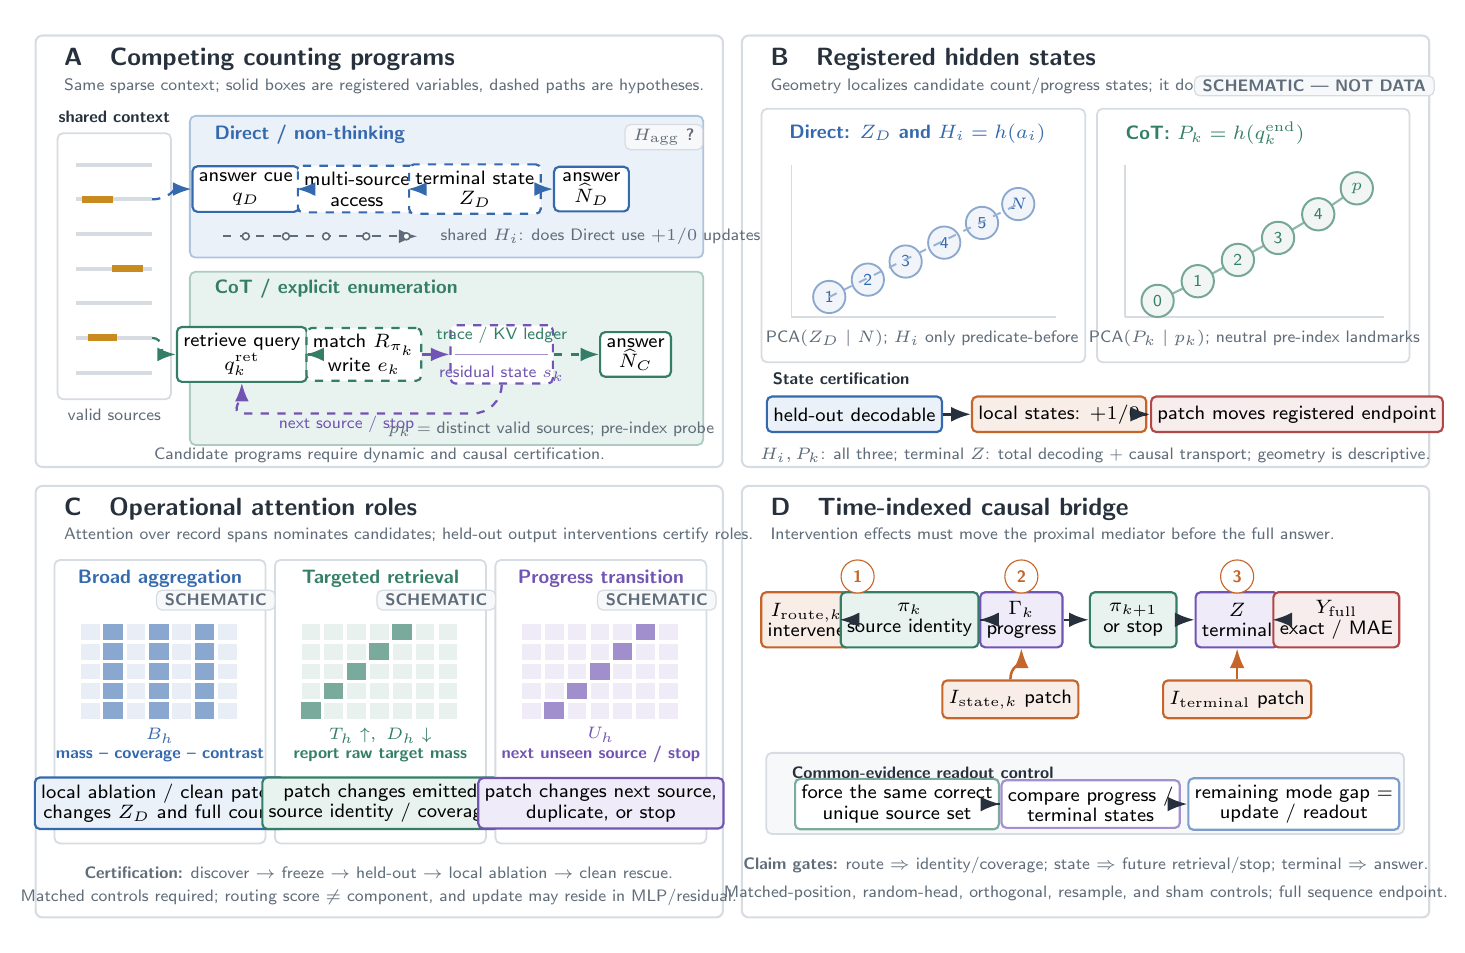
\begin{tikzpicture}[x=1cm,y=1cm]
\path[use as bounding box] (0,0) rectangle (17.90,11.40);

% Panel frames
\draw[panel] (0.10,5.82) rectangle (8.83,11.30);
\draw[panel] (9.07,5.82) rectangle (17.80,11.30);
\draw[panel] (0.10,0.10) rectangle (8.83,5.58);
\draw[panel] (9.07,0.10) rectangle (17.80,5.58);

% ==========================================================================
% A. Candidate computations
\node[title] at (0.34,11.00) {\textbf{A}\quad Competing counting programs};
\node[subtitle] at (0.34,10.66)
  {Same sparse context; solid boxes are registered variables, dashed paths are hypotheses.};

\node[small,font=\bfseries\fontsize{6.5}{7.3}\selectfont] at (1.10,10.27)
  {shared context};
\draw[subpanel] (0.38,6.68) rectangle (1.82,10.06);
\foreach \yy in {7.02,7.46,7.90,8.34,8.78,9.22,9.66}{
  \draw[grid,line width=1.45pt] (0.61,\yy) -- (1.58,\yy);
}
\draw[goldline,line width=2.5pt] (0.76,7.46) -- (1.14,7.46);
\draw[goldline,line width=2.5pt] (1.07,8.34) -- (1.47,8.34);
\draw[goldline,line width=2.5pt] (0.69,9.22) -- (1.08,9.22);
\node[tiny] at (1.10,6.48) {valid sources};

% Direct lane
\draw[lane,draw=direct!40,fill=directlight] (2.06,8.48) rectangle (8.58,10.28);
\node[font=\bfseries\fontsize{7.2}{8.0}\selectfont,text=direct,anchor=west]
  at (2.25,10.04) {Direct / non-thinking};
\node[badge] at (8.08,10.01) {$H_{\mathrm{agg}}$ ?};

\node[nodebase,draw=direct,fill=white,minimum width=.92cm] (aqd) at (2.77,9.35)
  {answer cue\\$q_D$};
\node[nodebase,draw=direct,dashed,fill=white,minimum width=1.26cm] (aagg) at (4.18,9.35)
  {multi-source\\access};
\node[nodebase,draw=direct,dashed,fill=white,minimum width=1.03cm] (azd) at (5.68,9.35)
  {terminal state\\$Z_D$};
\node[nodebase,draw=direct,fill=white,minimum width=.95cm] (aad) at (7.16,9.35)
  {answer\\$\widehat N_D$};
\draw[candidate,draw=direct] (1.58,9.22) to[out=0,in=180] (aqd.west);
\draw[candidate,draw=direct] (aqd) -- (aagg);
\draw[candidate,draw=direct] (aagg) -- (azd);
\draw[candidate,draw=direct] (azd) -- (aad);

\draw[candidate] (2.48,8.75) -- (4.95,8.75);
\foreach \xx in {2.77,3.28,3.79,4.30,4.81}{
  \draw[draw=muted,fill=white,line width=.58pt] (\xx,8.75) circle (1.25pt);
}
\node[tiny,anchor=west] at (5.12,8.75)
  {shared $H_i$: does Direct use $+1/0$ updates?};

% CoT lane
\draw[lane,draw=cot!40,fill=cotlight] (2.06,6.10) rectangle (8.58,8.30);
\node[font=\bfseries\fontsize{7.2}{8.0}\selectfont,text=cot,anchor=west]
  at (2.25,8.08) {CoT / explicit enumeration};
\node[nodebase,draw=cot,fill=white,minimum width=.88cm] (aqk) at (2.72,7.25)
  {retrieve query\\$q_k^{\rm ret}$};
\node[nodebase,draw=cot,dashed,fill=white,minimum width=1.28cm] (awrite) at (4.27,7.25)
  {match $R_{\pi_k}$\\write $e_k$};
\node[nodebase,draw=transition,dashed,fill=white,minimum width=1.30cm,
      minimum height=.74cm] (agamma) at (6.02,7.25) {};
\draw[transition!65,line width=.52pt] (5.43,7.25) -- (6.61,7.25);
\node[font=\fontsize{5.9}{6.6}\selectfont,text=cot] at (6.02,7.49)
  {trace / KV ledger};
\node[font=\fontsize{5.9}{6.6}\selectfont,text=transition] at (6.02,7.01)
  {residual state $s_k$};
\node[nodebase,draw=cot,fill=white,minimum width=.86cm] (aac) at (7.72,7.25)
  {answer\\$\widehat N_C$};
\draw[candidate,draw=cot] (1.58,7.46) to[out=0,in=180] (aqk.west);
\draw[candidate,draw=cot] (aqk) -- (awrite);
\draw[candidate,draw=transition] (awrite) -- (agamma);
\draw[candidate,draw=cot] (agamma) -- (aac);
\draw[candidate,draw=transition] (agamma.south)
  to[out=-90,in=0] (5.65,6.50) -- (2.72,6.50)
  to[out=180,in=-90] (aqk.south);
\node[tiny,text=transition] at (4.05,6.36) {next source / stop};
\node[tiny] at (6.65,6.30) {$p_k$ = distinct valid sources; pre-index probe};
\node[tiny] at (4.47,5.97)
  {Candidate programs require dynamic and causal certification.};

% ==========================================================================
% B. Registered hidden states
\node[title] at (9.31,11.00) {\textbf{B}\quad Registered hidden states};
\node[subtitle] at (9.31,10.66)
  {Geometry localizes candidate count/progress states; it does not establish their use.};

\draw[subpanel] (9.32,7.15) rectangle (13.43,10.37);
\draw[subpanel] (13.58,7.15) rectangle (17.55,10.37);
\node[badge] at (16.34,10.66) {SCHEMATIC --- NOT DATA};
\node[font=\bfseries\fontsize{6.9}{7.7}\selectfont,text=direct,anchor=west]
  at (9.55,10.06) {Direct: $Z_D$ and $H_i=h(a_i)$};
\node[font=\bfseries\fontsize{6.9}{7.7}\selectfont,text=cot,anchor=west]
  at (13.82,10.06) {CoT: $P_k=h(q_k^{\rm end})$};

% Direct analysis template
\draw[grid,line width=.62pt] (9.70,7.73) -- (9.70,9.66);
\draw[grid,line width=.62pt] (9.70,7.73) -- (13.06,7.73);
\foreach \x/\y/\lab in {10.18/7.98/1,10.67/8.20/2,11.15/8.43/3,
                         11.64/8.67/4,12.12/8.92/5,12.58/9.16/$N$}{
  \draw[direct!58,fill=direct!7,line width=.66pt] (\x,\y) circle (2.05mm);
  \node[font=\fontsize{5.8}{6.4}\selectfont,text=direct] at (\x,\y) {\lab};
}
\draw[direct!52,dashed,line width=.70pt] (10.18,7.98) -- (12.58,9.16);
\node[tiny] at (11.36,7.46) {PCA$(Z_D\mid N)$; $H_i$ only predicate-before};

% CoT analysis template
\draw[grid,line width=.62pt] (13.94,7.73) -- (13.94,9.66);
\draw[grid,line width=.62pt] (13.94,7.73) -- (17.22,7.73);
\draw[cot!55,line width=.78pt] (14.35,7.93) -- (14.86,8.18) -- (15.37,8.45)
  -- (15.88,8.73) -- (16.39,9.03) -- (16.88,9.36);
\foreach \x/\y/\lab in {14.35/7.93/0,14.86/8.18/1,15.37/8.45/2,
                         15.88/8.73/3,16.39/9.03/4,16.88/9.36/$p$}{
  \draw[cot!68,fill=cot!7,line width=.72pt] (\x,\y) circle (2.05mm);
  \node[font=\fontsize{5.8}{6.4}\selectfont,text=cot] at (\x,\y) {\lab};
}
\node[tiny] at (15.58,7.46) {PCA$(P_k\mid p_k)$; neutral pre-index landmarks};

\node[small,font=\bfseries\fontsize{6.2}{7.0}\selectfont,anchor=west]
  at (9.34,6.94) {State certification};
\node[nodebase,draw=direct,fill=directlight,minimum width=2.06cm,minimum height=.45cm]
  (bdecode) at (10.50,6.49) {held-out decodable};
\node[nodebase,draw=intervention,fill=interventionlight,minimum width=2.18cm,minimum height=.45cm]
  (bdynamic) at (13.10,6.49) {local states: $+1/0$};
\node[nodebase,draw=errorred,fill=errorlight,minimum width=2.62cm,minimum height=.45cm]
  (bcausal) at (16.12,6.49) {patch moves registered endpoint};
\draw[flow] (bdecode) -- (bdynamic);
\draw[flow] (bdynamic) -- (bcausal);
\node[tiny] at (13.56,5.97)
  {$H_i,P_k$: all three; terminal $Z$: total decoding + causal transport; geometry is descriptive.};

% ==========================================================================
% C. Attention candidates
\node[title] at (0.34,5.29) {\textbf{C}\quad Operational attention roles};
\node[subtitle] at (0.34,4.95)
  {Attention over record spans nominates candidates; held-out output interventions certify roles.};

\draw[subpanel] (0.34,1.04) rectangle (3.02,4.64);
\draw[subpanel] (3.14,1.04) rectangle (5.82,4.64);
\draw[subpanel] (5.94,1.04) rectangle (8.62,4.64);

\node[font=\bfseries\fontsize{6.7}{7.5}\selectfont,text=direct] at (1.68,4.40)
  {Broad aggregation};
\node[font=\bfseries\fontsize{6.7}{7.5}\selectfont,text=cot] at (4.48,4.40)
  {Targeted retrieval};
\node[font=\bfseries\fontsize{6.7}{7.5}\selectfont,text=transition] at (7.28,4.40)
  {Progress transition};
\node[badge] at (2.39,4.13) {SCHEMATIC};
\node[badge] at (5.19,4.13) {SCHEMATIC};
\node[badge] at (7.99,4.13) {SCHEMATIC};

% Base heatmap grids
\foreach \rr in {0,...,4}{
  \foreach \cc in {0,...,6}{
    \fill[direct!11] ({0.67+0.29*\cc},{2.62+0.25*\rr}) rectangle ++(.25,.21);
    \draw[white,line width=.24pt] ({0.67+0.29*\cc},{2.62+0.25*\rr}) rectangle ++(.25,.21);
    \fill[cot!11] ({3.47+0.29*\cc},{2.62+0.25*\rr}) rectangle ++(.25,.21);
    \draw[white,line width=.24pt] ({3.47+0.29*\cc},{2.62+0.25*\rr}) rectangle ++(.25,.21);
    \fill[transition!11] ({6.27+0.29*\cc},{2.62+0.25*\rr}) rectangle ++(.25,.21);
    \draw[white,line width=.24pt] ({6.27+0.29*\cc},{2.62+0.25*\rr}) rectangle ++(.25,.21);
  }
}
% Broad columns
\foreach \rr in {0,...,4}{
  \foreach \cc in {1,3,5}{
    \fill[direct!58] ({0.67+0.29*\cc},{2.62+0.25*\rr}) rectangle ++(.25,.21);
  }
}
% Matched diagonal
\foreach \cc/\rr in {0/0,1/1,2/2,3/3,4/4}{
  \fill[cot!66] ({3.47+0.29*\cc},{2.62+0.25*\rr}) rectangle ++(.25,.21);
}
% Next-source offset
\foreach \cc/\rr in {1/0,2/1,3/2,4/3,5/4}{
  \fill[transition!66] ({6.27+0.29*\cc},{2.62+0.25*\rr}) rectangle ++(.25,.21);
}

\node[small,font=\bfseries\fontsize{6.4}{7.1}\selectfont,text=direct] at (1.68,2.29)
  {$B_h$\\mass -- coverage -- contrast};
\node[small,font=\bfseries\fontsize{6.4}{7.1}\selectfont,text=cot] at (4.48,2.29)
  {$T_h\uparrow,\ D_h\downarrow$\\report raw target mass};
\node[small,font=\bfseries\fontsize{6.4}{7.1}\selectfont,text=transition] at (7.28,2.29)
  {$U_h$\\next unseen source / stop};

\node[nodebase,draw=direct,fill=directlight,minimum width=2.16cm,minimum height=.64cm]
  at (1.68,1.55) {local ablation / clean patch\\changes $Z_D$ and full count};
\node[nodebase,draw=cot,fill=cotlight,minimum width=2.16cm,minimum height=.64cm]
  at (4.48,1.55) {patch changes emitted\\source identity / coverage};
\node[nodebase,draw=transition,fill=transitionlight,minimum width=2.16cm,minimum height=.64cm]
  at (7.28,1.55) {patch changes next source,\\duplicate, or stop};

\node[tiny] at (4.46,0.67)
  {\textbf{Certification:} discover $\rightarrow$ freeze $\rightarrow$ held-out
   $\rightarrow$ local ablation $\rightarrow$ clean rescue.};
\node[tiny] at (4.46,0.36)
  {Matched controls required; routing score $\neq$ component, and update may reside in MLP/residual.};

% ==========================================================================
% D. Time-indexed causal bridge
\node[title] at (9.31,5.29) {\textbf{D}\quad Time-indexed causal bridge};
\node[subtitle] at (9.31,4.95)
  {Intervention effects must move the proximal mediator before the full answer.};

\node[nodebase,draw=intervention,fill=interventionlight,minimum width=1.02cm,
      minimum height=.70cm] (diroute) at (9.89,3.88)
  {$I_{{\rm route},k}$\\intervene};
\node[nodebase,draw=cot,fill=cotlight,minimum width=1.18cm,
      minimum height=.70cm] (dsource) at (11.20,3.88)
  {$\pi_k$\\source identity};
\node[nodebase,draw=transition,fill=transitionlight,minimum width=1.04cm,
      minimum height=.70cm] (dstate) at (12.62,3.88)
  {$\Gamma_k$\\progress};
\node[nodebase,draw=cot,fill=cotlight,minimum width=1.10cm,
      minimum height=.70cm] (dnext) at (14.04,3.88)
  {$\pi_{k+1}$\\or stop};
\node[nodebase,draw=transition,fill=transitionlight,minimum width=.70cm,
      minimum height=.70cm] (dz) at (15.36,3.88)
  {$Z$\\terminal};
\node[nodebase,draw=errorred,fill=errorlight,minimum width=1.12cm,
      minimum height=.70cm] (dy) at (16.62,3.88)
  {$Y_{\rm full}$\\exact / MAE};
\draw[flow] (diroute) -- (dsource);
\draw[flow] (dsource) -- (dstate);
\draw[flow] (dstate) -- (dnext);
\draw[flow] (dnext) -- (dz);
\draw[flow] (dz) -- (dy);

\node[nodebase,draw=intervention,fill=interventionlight,minimum width=1.28cm,
      minimum height=.48cm] (distate) at (12.48,2.87) {$I_{{\rm state},k}$ patch};
\node[nodebase,draw=intervention,fill=interventionlight,minimum width=1.30cm,
      minimum height=.48cm] (diterm) at (15.36,2.87) {$I_{\rm terminal}$ patch};
\draw[flow,draw=intervention] (distate.north) to[out=90,in=-90] (dstate.south);
\draw[flow,draw=intervention] (diterm.north) to[out=90,in=-90] (dz.south);
\node[interventionmark] at (10.54,4.43) {1};
\node[interventionmark] at (12.62,4.43) {2};
\node[interventionmark] at (15.36,4.43) {3};

\draw[subpanel,fill=panelgray] (9.38,1.16) rectangle (17.48,2.19);
\node[small,font=\bfseries\fontsize{6.5}{7.3}\selectfont,anchor=west] at (9.58,1.94)
  {Common-evidence readout control};
\node[nodebase,draw=cot!65,fill=white,minimum width=1.80cm] (dfix) at (11.04,1.54)
  {force the same correct\\unique source set};
\node[nodebase,draw=transition!65,fill=white,minimum width=1.76cm] (dcompare) at (13.50,1.54)
  {compare progress /\\terminal states};
\node[nodebase,draw=direct!65,fill=white,minimum width=1.92cm] (dgap) at (16.08,1.54)
  {remaining mode gap =\\update / readout};
\draw[flow] (dfix) -- (dcompare);
\draw[flow] (dcompare) -- (dgap);

\node[tiny] at (13.44,0.76)
  {\textbf{Claim gates:} route $\Rightarrow$ identity/coverage; state $\Rightarrow$ future retrieval/stop;
   terminal $\Rightarrow$ answer.};
\node[tiny] at (13.44,0.40)
  {Matched-position, random-head, orthogonal, resample, and sham controls; full sequence endpoint.};

\end{tikzpicture}
\end{document}
